% two color theme fdu_red and fdu_blue, choose your preference main document and switch in the menu
% github repo https://github.com/milanmarks/FDU-Beamer-Theme
\documentclass{beamer}
\usepackage{ctex, hyperref}
\usepackage[T1]{fontenc}

% other packages
\usepackage{latexsym,amsmath,xcolor,multicol,booktabs,calligra,multirow}
\usepackage{graphicx,pstricks,listings,stackengine}

\author{陈纳川、王子卿、张涵石、吴信岩}
\title{基于机器学习算法的多因子选股策略}
\subtitle{Machine Learning-Based Multi-Factor Strategy in A-Shares}
\institute{中国人民大学财政金融学院}
\date{2025年12月8日}
\usepackage{RenminUniv}

% defs
\def\cmd#1{\texttt{\color{red}\footnotesize $\backslash$#1}}
\def\env#1{\texttt{\color{blue}\footnotesize #1}}
\definecolor{deepblue}{rgb}{0,0,0.5}
\definecolor{deepred}{rgb}{0.6,0,0}
\definecolor{deepgreen}{rgb}{0,0.5,0}
\definecolor{halfgray}{gray}{0.55}

% helper for footer quote (theme macro missing in some setups)
\newcommand{\footquote}[1]{\footnotesize #1}

\lstset{
    basicstyle=\ttfamily\small,
    keywordstyle=\bfseries\color{deepblue},
    emphstyle=\ttfamily\color{deepred},    % Custom highlighting style
    stringstyle=\color{deepgreen},
    numbers=left,
    numberstyle=\small\color{halfgray},
    rulesepcolor=\color{red!20!green!20!blue!20},
    frame=shadowbox,
}


\begin{document}

\kaishu
\begin{frame}
    \titlepage
    \begin{figure}[htpb]
        \begin{center}
            \includegraphics[width=0.4\linewidth]{pic/Renmin_Univ_Logo.eps}
        \end{center}
    \end{figure}
\end{frame}

\begin{frame}{项目概况}
    本项目构建了一个多因子库,并使用机器学习方法(随机森林和 XGBoost)将因子作为特征进行选股。随后对以上策略使用多种指标和基准模型进行检验和收益归因,验证了该策略取得了显著的超额收益,并且稳健性较高。
    \begin{figure}
        \centering
        % width 设为 \textwidth 的 0.8 到 0.9 倍最合适
        \includegraphics[width=0.9\textwidth]{pic/strategy_performance.pdf}
    \end{figure}
\end{frame}

\begin{frame}{目录}
    \tableofcontents[hideallsubsections]
\end{frame}


\section{数据来源及预处理}
\subsection{数据来源}

\begin{frame}{数据来源}
    \begin{itemize}
        \item 数据来源:Tushare API
        \item 数据范围:2000 年 1 月至 2025 年 11 月
        \item 数据内容:
        \begin{itemize}
            \item 个股行情数据(开盘价、收盘价、最高价、最低价、成交量等)
            \item 指数行情数据(上证综指、深证成指、沪深300等)
            \item 行业分类数据(申万行业分类)
            \item 财务报表数据(资产负债表、利润表、现金流量表等)
            \item 宏观经济数据(GDP、CPI、利率等)
        \end{itemize}
    \end{itemize}
\end{frame}

\subsection{数据预处理}

\begin{frame}{数据预处理}
    \begin{enumerate}
        \item 使用日频个股行情和复权因子,计算复权后的每日收益率
        \item 频率对齐:将日频和季度数据转化为月频,计算相关指标
        \begin{itemize}
            \item 按照财报发布日,填充季度数据,避免数据泄露
            \item 修正了财报YTD数据重复计算的问题
            \item 使用月度的开盘价和收盘价计算月度收益率
        \end{itemize}
        \item 股票池筛选:建立一个白名单,过滤一下风险过大的股票
        \begin{itemize}
            \item ST 股、上市未满一年的次新股和停牌的股票
            \item 市值分位数小于 30\% 的股票(壳价值)
            \item 涨停板等无法在调仓日无法买入的股票
        \end{itemize}
    \end{enumerate}
\end{frame}

\section{因子库的构建和筛选}

\begin{frame}{因子库的构建和筛选}
    因子主要分为技术面和基本面两个大类,各分多个小类:
    \begin{enumerate}
        \item 技术面因子:
        \begin{itemize}
            \item 技术因子
            \item 动量因子
            \item 波动率因子
            \item 流动性因子
        \end{itemize}
        \item 基本面因子:
        \begin{itemize}
            \item 质量因子
            \item 价值因子
            \item 成长因子
            \item 规模因子
        \end{itemize}
    \end{enumerate}
    对因子的 IC、ICIR 以及分组回测指标进行筛选,最终选取了 99 个因子用于后续的模型训练。

    其中包含39 个基本面因子,60 个技术面因子
\end{frame}


\section{机器学习策略构建}
\subsection{XGBoost 模型}

\begin{frame}{XGBoost 模型简介}
    XGBoost(极端梯度提升)算法是一种基于 Boosting 框架,串行训练 $K$ 棵分类回归树 (CART)的集成学习算法。
    通过在每一棵新树 $f_k$ 都在拟合上一轮预测的残差,逐步逼近真实值。
    $$\hat{y}_i^{(t)} = \sum_{k=1}^t f_k(x_i) = \hat{y}_i^{(t-1)} + f_t(x_i)$$
相比传统的树算法,XGBoost 在目标函数中引入了显式的正则化项:
$$\text{Obj} = \sum_{i=1}^n l(y_i, \hat{y}_i) + \sum_{k=1}^K \Omega(f_k)$$
 \begin{itemize}
        \item $l$: 损失函数 (如 MSE),衡量预测准确度。
        \item $\Omega(f_k) = \gamma T + \frac{1}{2}\lambda ||w||^2$: 正则项,惩罚树的复杂度(叶子节点数 $T$)和权重 ($w$),有效防止过拟合。
    \end{itemize}
\end{frame}

\begin{frame}{XGBoost策略构建}
    模型选择动机
    \begin{itemize}
        \item 捕捉非线性:可以捕捉到因子和收益率之间的非线性关系
        \item 挖掘交互项:可以捕捉到不同因子之间的复杂非线性关系
    \end{itemize}
    训练与预测机制
    \begin{itemize}
        \item 滚动窗口
        \begin{itemize}
            \item 训练集: 过去 24 个月的数据。
            \item 验证集: 紧邻的下一个月的收益率$R_{i, t+1}$
        \end{itemize}
        \item 目标函数:最大化收益率
        \item 特征: 经过标准化和去极值处理的因子库
        \item 关键超参数:1000 棵树,最大深度 6 层,学习率 0.05
    \end{itemize}

    \begin{figure}
        \centering
        % 这里可以插入一个简单的滚动窗口示意图,或者使用 tikz 画一个
        % \includegraphics[width=0.8\textwidth]{images/rolling_window.pdf}
        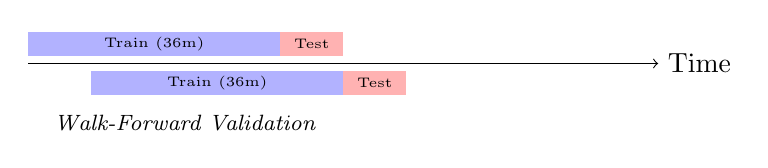
\begin{tikzpicture}[xscale=0.8, yscale=0.5]
            \draw[->] (0,0) -- (10,0) node[right] {Time};
            \fill[blue!30] (0,0.2) rectangle (4,0.8) node[midway, black] {\tiny Train (36m)};
            \fill[red!30] (4,0.2) rectangle (5,0.8) node[midway, black] {\tiny Test};
            \fill[blue!30] (1,-0.8) rectangle (5,-0.2) node[midway, black] {\tiny Train (36m)};
            \fill[red!30] (5,-0.8) rectangle (6,-0.2) node[midway, black] {\tiny Test};
            \node at (2.5, -1.5) {\footnotesize \textit{Walk-Forward Validation}};
        \end{tikzpicture}
    \end{figure}
    
\end{frame}


\subsection{随机森林模型}

\begin{frame}{随机森林模型简介}
    随机森林是一种集成学习方法,通过构建多个决策树并结合其预测结果,提高模型的准确性和鲁棒性。与 XGBoost 的串行优化不同,RF 采用并行训练。\\
    其特点是双重随机性
    \begin{itemize}
        \item 样本随机: 有放回地随机采样
        \item 特征随机: 在节点分裂时,只考虑特征子集
    \end{itemize}
    回归问题取所有树的平均值,分类问题取投票。其优势在于其极高的稳定性和抗过拟合能力。模型的方差由单棵树的方差 ($\sigma^2$) 和树之间的相关性 ($\rho$) 决定:
$$\text{Var}(\text{Ensemble}) = \rho \sigma^2 + \frac{1-\rho}{K} \sigma^2$$
\end{frame}
\begin{frame}{随机森林策略构建}
    模型选择动机
    \begin{itemize}
        \item 抗过拟合:A 股市场充斥着大量随机噪音,RF 更不容易过拟合
        \item 非线性与交互: 能够捕捉因子间的非线性关系和交互作用
        \item 特征重要性: 利用 OOB 数据进行特征重要性排序,可以进行因子筛选
    \end{itemize}
    训练与预测机制
    \begin{itemize}
        \item 滚动窗口
        \begin{itemize}
            \item 训练集: 过去 24 个月的数据。
            \item 验证集: 紧邻的下一个月的收益率$R_{i, t+1}$
        \end{itemize}
        \item 目标函数:最大化收益率
        \item 特征: 经过标准化和去极值处理的因子库
        \item 关键超参数:100 棵树,最大深度 6 层,叶节点最小样本: 20
    \end{itemize}
\end{frame}

\section{策略检验和收益归因}
\subsection{主要指标汇总}
\begin{frame}{策略表现: 累计收益曲线}
    % 上方:文字分析
    \begin{itemize}
        \item 长期显著跑赢基准:策略在回测区间内持续产生超额收益,市值加权累计收益约 200 倍。
        \item 风格效应分析:等权累计收益超 3000 倍,反映 A 股小市值因子红利与复利效应叠加。
    \end{itemize}

    % 下方:插入宽图
    \begin{figure}
        \centering
        % 宽度设为页面宽度的 95%,高度限制在页面的 55%,保证图表尽量大且不变形
        \includegraphics[width=0.95\textwidth]{pic/strategy_performance.pdf}
        \caption{\footnotesize 策略累计净值走势(2000 年 1 月 - 2025 年 11 月)}
    \end{figure}
\end{frame}

\begin{frame}{核心绩效指标}
    1. 核心绩效指标对比 (2000 - 2025 Long-Only)
    
    \begin{table}[]
        \centering
        \renewcommand{\arraystretch}{1.2}
        \resizebox{\textwidth}{!}{% 自动缩放表格以适应宽度
        \begin{tabular}{l|cc|cc|c}
        \hline
        \multirow{2}{*}{\textbf{Indicator}} & \multicolumn{2}{c|}{\textbf{Random Forest (RF)}} & \multicolumn{2}{c|}{\textbf{XGBoost (XGB)}} & \textbf{Benchmark} \\ \cline{2-6} 
         & \textbf{VW} & \textbf{EW} & \textbf{VW} & \textbf{EW} & \textit{CSI 500} \\ \hline
        \textbf{Ann. Return} & 23.16\% & 33.49\% & 22.17\% & 35.27\% & $\sim$8.5\% \\ 
        \textbf{Sharpe Ratio} & 0.8618 & 1.1374 & 0.7488 & 1.1317 & 0.35 \\ 
        \textbf{Max Drawdown} & -64.49\% & -62.61\% & -74.68\% & -65.04\% & -72.0\% \\ 
        \textbf{Win Rate} & 60.70\% & 62.81\% & 60.70\% & 63.16\% & 52.1\% \\ \hline
        \end{tabular}
        }
    \end{table}
    2. 模型特性分析
    \begin{itemize}
        \item 权重影响: 
        \textit{EW 策略普遍优于 VW,表明模型在中小市值股票上的选股能力更为显著}
        
        \item 模型差异: 
        \textit{XGBoost在 EW中收益率更高,体现了其对非线性 Alpha 的挖掘潜力;而 Random Forest回撤控制更优,表现出更强的抗噪性与稳健性。}
    \end{itemize}
\end{frame}

\begin{frame}{主要指标汇总: 有效性分析}


    \begin{columns}
        % 左侧:累计 IC
        \column{0.48\textwidth}
        \centering
        \begin{figure}
            \IfFileExists{pic/cumulative_ic.pdf}{%
                \includegraphics[width=0.9\textwidth]{pic/cumulative_ic.pdf}%
            }{\fbox{\strut Missing file: pic/cumulative_ic.pdf}}
        \end{figure}
        \vspace{-0.2cm}
        \footnotesize
        \begin{itemize}
            \item \textbf{趋势}: 曲线呈近乎线性的上升趋势。
            \item \textbf{回撤}: 历史上未出现显著的长期回撤,适应多种市场风格。
        \end{itemize}

        % 右侧:移动平均 IC
        \column{0.48\textwidth}
        \begin{figure}
            \centering
            \IfFileExists{pic/rolling_ic.pdf}{%
                \includegraphics[width=0.9\textwidth]{pic/rolling_ic.pdf}%
            }{\fbox{\strut Missing file: pic/rolling_ic.pdf}}
        \end{figure}
        \vspace{-0.2cm}
        \footnotesize
        \begin{itemize}
            \item \textbf{稳定性}: 滚动均值长期位于 0 轴上方,极少击穿安全线。
            \item \textbf{高信噪比}: \textbf{ICIR > 1.0} 表现优秀。
        \end{itemize}
    \end{columns}
\end{frame}


\subsection{CH3\&CH4模型分析}
\begin{frame}{CH3\&CH4模型分析: Random Forest (RF)}
    \begin{itemize}
        \item \textbf{CH-3}: 
$$R_{p} = \alpha + \beta_{MKT} R_{MKT} + \beta_{SMB} R_{SMB} + \beta_{VMG} R_{VMG} + \epsilon$$
        \item \textbf{CH-4}: 
$$R_{p} = \alpha' + \beta_{MKT} R_{MKT} + \beta_{SMB} R_{SMB} + \beta_{VMG} R_{VMG} + \beta_{PMO} R_{PMO} + \epsilon$$
    \end{itemize}

    \begin{table}[]
        \centering
        \renewcommand{\arraystretch}{1.2}
        \resizebox{\textwidth}{!}{%
        \begin{tabular}{l|ccc|ccc}
        \hline
        \multirow{2}{*}{\textbf{Strategy}} & \multicolumn{3}{c|}{\textbf{CH-3 Model}} & \multicolumn{3}{c}{\textbf{CH-4 Model}} \\ \cline{2-7} 
         & \textbf{Ann. Alpha} & \textbf{t-stat} & \textbf{$R^2$} & \textbf{Ann. Alpha} & \textbf{t-stat} & \textbf{$R^2$} \\ \hline
        \textbf{EW (等权)} & 32.78\% & \textbf{11.26} & 0.035 & 33.31\% & \textbf{11.23} & 0.042 \\ 
        \textbf{VW (市值加权)} & 19.43\% & \textbf{4.29} & 0.003 & 20.52\% & \textbf{4.45} & 0.009 \\ \hline
        \end{tabular}%
        }
    \end{table}

    \vspace{0.1cm}
    \textbf{结果解读:}
    \begin{itemize}
        \item RF 策略在 CH-3 和 CH-4 模型下均获得显著的 Alpha。
        \item VW 策略的年化 Alpha 依然达到 \textbf{20\%} 左右,证明收益并非主要来自风险因子暴露。
    \end{itemize}
\end{frame}

\begin{frame}{CH3\&CH4模型分析: XGBoost (XGB)}
    \begin{table}[]
        \centering
        \renewcommand{\arraystretch}{1.2}
        \resizebox{\textwidth}{!}{%
        \begin{tabular}{l|ccc|ccc}
        \hline
        \multirow{2}{*}{\textbf{Strategy}} & \multicolumn{3}{c|}{\textbf{CH-3 Model}} & \multicolumn{3}{c}{\textbf{CH-4 Model}} \\ \cline{2-7} 
         & \textbf{Ann. Alpha} & \textbf{t-stat} & \textbf{$R^2$} & \textbf{Ann. Alpha} & \textbf{t-stat} & \textbf{$R^2$} \\ \hline
        \textbf{EW (等权)} & 35.19\% & \textbf{13.44} & 0.043 & 36.50\% & \textbf{13.81} & 0.067 \\ 
        \textbf{VW (市值加权)} & 23.32\% & \textbf{5.36} & 0.022 & 25.07\% & \textbf{5.67} & 0.034 \\ \hline
        \end{tabular}%
        }
    \end{table}

    \vspace{0.2cm}

    \begin{itemize}
        \item \textbf{Alpha 显著性}: 两个模型在引入动量因子 (CH-4) 后,Alpha 依然显著且甚至略有提升,说明策略不仅仅是捕捉了动量效应。
        \item \textbf{XGB 优势}: XGBoost 在 VW 组合下的 Alpha t-stat 达到 \textbf{5.67} ,表明其在大资金容量下的选股确定性更高,更有效地剥离了常见的风险因子。
        \item \textbf{低 $R^2$}: 极低的 $R^2$ (不到 0.1) 说明策略收益与常见风格因子相关性极低,具备独特的特质收益源。
    \end{itemize}
\end{frame}

\subsection{Fama-MacBeth回归分析}

\begin{frame}{Fama-MacBeth 横截面回归分析}

    \begin{itemize}
        \item \textbf{回归方程} (每月 $t$ 进行横截面回归):
        \begin{equation*}
            R_{i, t+1} = \lambda_0 + \lambda_{ML} \cdot \hat{y}_{i,t} + \lambda_{Size} \cdot \text{Size}_{i,t} + \lambda_{Bm} \cdot \text{Bm}_{i,t} + \dots + \epsilon_{i,t}
        \end{equation*}
        \item \textbf{控制变量}: 市值, 账面市值比, 12个月动量, 非流动性。
    \end{itemize}
    \begin{table}[]
        \centering
        \renewcommand{\arraystretch}{1.2}
        \resizebox{\textwidth}{!}{%
        \begin{tabular}{l|cc|cc}
        \hline
        \multirow{2}{*}{\textbf{Factor}} & \multicolumn{2}{c|}{\textbf{XGBoost (XGB)}} & \multicolumn{2}{c}{\textbf{Random Forest (RF)}} \\ \cline{2-5} 
         & \textbf{Coeff ($\lambda$)} & \textbf{t-stat} & \textbf{Coeff ($\lambda$)} & \textbf{t-stat} \\ \hline
        \textbf{Intercept} & -0.0544 & -8.46 & -0.1145 & -13.49 \\ 
        \textbf{Model Score (\texttt{pred\_ret})} & \textbf{0.1363} & \textbf{18.22} & \textbf{0.2559} & \textbf{21.24} \\ \hline
        \end{tabular}%
        }
    \end{table}

    \textbf{结论:}
    \begin{itemize}
        \item 两个模型的预测分数$t$值均远超临界值,分别为 \textbf{18.22} 和 \textbf{21.24},表明其具有极强的独立预测能力。
        \item 即使在控制了显著的\textbf{小市值效应} ($\lambda_{Size} < 0$) 后,机器学习因子的显著性依然未被削弱。
    \end{itemize}
\end{frame}

\subsection{GRS检验}
\begin{frame}{GRS 联合显著性检验}
    \begin{itemize}
        \item \textbf{目的}: 检验 5 组投资组合 (Q1 $\sim$ Q5) 的定价误差 ($\alpha$) 是否\textbf{联合为零}。
        \item \textbf{零假设 ($H_0$)}: $\alpha_{Q1} = \alpha_{Q2} = \alpha_{Q3} = \alpha_{Q4} = \alpha_{Q5} = 0$
        \item \textbf{基准模型}: Fama-French 三因子模型 (CH-3)。
    \end{itemize}
    \begin{table}[]
        \centering
        \renewcommand{\arraystretch}{1.3}
        \begin{tabular}{l|c|c|c}
        \hline
        Model & GRS Statistic & P-Value & Result \\ \hline
        Random Forest (RF) & 5.64 & 0.0001 & Reject $H_0$ \\ 
        XGBoost (XGB) & 7.22 & < 0.0001 & Reject $H_0$ \\ \hline
        \end{tabular}
    \end{table}
    \begin{alertblock}{结论}
        \begin{itemize}
            \item \textbf{统计学意义}: 强烈拒绝零假设。这证明 Q1-Q5 组合中存在无法被市场、市值和价值因子解释的显著 Alpha。
            \item \textbf{经济学意义}: 机器学习模型确实挖掘到了独立于传统因子之外的有效选股逻辑。
        \end{itemize}
    \end{alertblock}
\end{frame}
\subsection{CNE-6模型和行业收益归因}
\begin{frame}{CNE-6 模型与行业收益归因}
    \begin{itemize}
        \item \textbf{回归方程} (每月横截面回归):
        \begin{equation*}
            R_{i, t+1} = \gamma_{ML} \cdot \hat{y}_{i,t} + \sum_{k=1}^{10} \gamma_{Style, k} \cdot F_{Style, k} + \sum_{j=1}^{110} \gamma_{Ind, j} \cdot D_{Ind, j} + \epsilon_{i,t}
        \end{equation*}
        \item 控制变量: 10个 Barra 因子 + 110个申万行业变量
    \end{itemize}

    \begin{columns}
        % 左侧:核心统计表
        \column{0.45\textwidth}
        \begin{table}[]
            \centering
            \renewcommand{\arraystretch}{1.1}
            \resizebox{\textwidth}{!}{%
            \begin{tabular}{l|c|c}
            \hline
            Factor & Return ($\gamma$) & t-stat \\ \hline
            ML Score & 22.80\% & 20.65 \\ \hline
            Size & -1.14\% & -7.59 \\ 
            Momentum & 0.17\% & 2.30 \\ 
            Liquidity & -0.46\% & -4.31 \\ 
            Earnings Yield & 0.25\% & 3.90 \\ 
            Beta & 0.17\% & 2.07 \\ \hline
            \end{tabular}%
            }
        \end{table}

        % 右侧:累计纯收益图
        \column{0.55\textwidth}
        结论:\\
        在剥离了所有风格和行业干扰后,ML 因子的纯收益 t-stat 高达 \textbf{20.65},证明策略拥有极其纯粹且显著的 \textbf{Alpha},而非简单的风格暴露。
    \end{columns}


\end{frame}
\section{总结与展望}

\section{参考文献}


\begin{frame}[allowframebreaks]
    \bibliography{ref}
    \bibliographystyle{alpha}
    % 如果参考文献太多的话,可以像下面这样调整字体:
    % \tiny\bibliographystyle{alpha}
\end{frame}

\begin{frame}
    \begin{center}
        {\Huge 请大家批评指正!}\\
    \end{center}
    \vfill % 推到底部
    \footquote{本项目代码已开源于 \textcolor{blue}{\url{https://github.com/nachuanchen/AMQI}}}\\
\end{frame}

\end{document}